\documentclass{article}

\usepackage[final]{neurips_2019}

\usepackage{xeCJK}
\setCJKmainfont{Noto Sans CJK TC}
% or another CJK font installed on your system

\usepackage{hyperref}
\usepackage{url}
\usepackage{booktabs}
\usepackage{amsfonts}
\usepackage{nicefrac}
\usepackage{microtype}
\usepackage{graphicx}
\usepackage{xcolor}
\usepackage{lipsum}

\newcommand{\note}[1]{\textcolor{blue}{{#1}}}

\title{
  NTU 2025 Fall Applied Deep Learning HW1 Report \\
  \vspace{1em}
  \small{\normalfont NTU CSIE 5431 Applied Deep Learning}
}

\author{
  CHIH-HAO LIAO \\
  School of Forestry and Resource Conservation\\
  Graduate Institute of Biomedical Electronics and Bioinformatics\\
  National Taiwan University\\
  \texttt{R11625015@ntu.edu.tw} \\
  % Examples of more authors
%   \And
%   Name \\
%   Department of Computer Science \\
%   Stanford University \\
%   \texttt{name@stanford.edu} \\
%   \And
%   Name \\
%   Department of Computer Science \\
%   Stanford University \\
%   \texttt{name@stanford.edu}
}

\begin{document}

\maketitle

\section{Report - Q1: Data processing (2\%)}
\subsection{Tokenizer (1\%)}
\begin{itemize}
    \item Describe in detail about the tokenization algorithm you use. You need to explain what algorithm does in your own ways. Just answering with “I called the () function” is not allowed.
\end{itemize}

In homework 1, we used the tokenizer from \texttt{hfl/chinese-lert-base}, which is based on the WordPiece subword algorithm. The key idea is to split text into subwords instead of whole words or only single characters. For Chinese words, where there are no spaces between words, the tokenizer looks for the longest possible subwords in its vocabulary. If a word is not found, it is broken into smaller and more frequent units until all characters are covered.

This method allows the model to handle rare or unseen words while keeping the vocabulary size manageable. The tokenizer outputs token IDs and also adds special symbols such as \texttt{[CLS]}, \texttt{[SEP]}, and \texttt{[PAD]}. These tokenized sequences are then used as the input for both multiple-choice validation (\texttt{Multiple choice}) and question answering validation (\texttt{Question answering}).

For example, when tokenizing the sentence pair "這是一個測試" and "這是一個測試", the tokenizer outputs:

\begin{verbatim}
{'input_ids':      [101, 6857, 3221, 671, 943, 3947, 6275, 102,
                    6857, 3221, 671, 943, 3947, 6275, 102],
 'token_type_ids': [0, 0, 0, 0, 0, 0, 0, 0, 1, 1, 1, 1, 1, 1, 1],
 'attention_mask': [1, 1, 1, 1, 1, 1, 1, 1, 1, 1, 1, 1, 1, 1, 1]}
\end{verbatim}

Here, \texttt{input\_ids} are the token IDs for each subword, \texttt{token\_type\_ids} distinguish the first and second sentences, and \texttt{attention\_mask} marks which tokens are real versus padding. In the code, the tokenized outputs are then un-flattened into batches of size 4 and the corresponding labels are added. This preprocessing ensures that the model can handle sentence pairs correctly and is ready for training, evaluation, or prediction on downstream tasks.

\subsection{Answer Span (1\%)}
\begin{itemize}
    \item How did you convert the answer span start/end position on characters to position on tokens after BERT tokenization?
    \item After your model predicts the probability of answer span start/end position, what rules did you apply to determine the final start/end position?
\end{itemize}

\vspace{1em}

\begin{itemize}
    \item \textbf{Converting character-level answer spans to token-level positions:}

          After loading the context for each question, we first obtained the start and end character positions of the answer within the context. Then, using the fast tokenizer from \texttt{hfl/chinese-lert-base}, we tokenized the question-context pair with \texttt{return\_offset\_mapping=True}. The offset mapping provides the start and end character indices for each token. For each answer, we identified the token whose offset range contains the start character of the answer as the token-level start position, and the token whose offset range contains the end character of the answer as the token-level end position. If the answer was not fully contained in the current tokenized span, the positions were set to the CLS token index.

    \item \textbf{Determining final answer span from model predictions:}

          After the model outputs the start and end logits for each token, we first select the tokens with the highest start and end probabilities as candidate positions. We then apply constraints:
          (1) the end position must not precede the start position,
          (2) the length of the predicted span must not exceed the \texttt{max\_answer\_length},
          and (3) if using \texttt{version\_2\_with\_negative}, the null score difference threshold is applied to decide if no answer should be returned. The final token-level start and end positions are then mapped back to the character positions in the context to extract the predicted answer text.
\end{itemize}

\section{Report - Q2: Modeling with BERTs and their variants (4\%)}

\subsection{Describe (2\%)}
\begin{itemize}
    \item \textbf{Your model}
          \begin{itemize}
              \item Multiple choice: hfl/chinese-lert-base
              \item Question answering: hfl/chinese-lert-base
          \end{itemize}
    \item \textbf{The performance of your model}
          \begin{itemize}
              \item Multiple choice: 0.9648
              \item Question answering: 83.5161
              \item Public Score: 0.77660
              \item Private Score: 0.81222
          \end{itemize}
    \item \textbf{The loss function you used}
          \begin{itemize}
              \item Multiple choice: CrossEntropyLoss
              \item Question answering: CrossEntropyLoss
          \end{itemize}
    \item \textbf{The optimization algorithm (e.g. Adam), learning rate and batch size}
          \begin{itemize}
              \item Multiple choice: AdamW, learning rate = 3e-5, batch size = 1 (training), 2 (evaluation)
              \item Question answering: AdamW, learning rate = 3e-5, batch size = 1 (training), 8 (evaluation)
          \end{itemize}
\end{itemize}

\subsection{Try another type of pre-trained LMs and describe (2\%)}
\begin{itemize}
    \item \textbf{The new model.}
    \item \textbf{The performance of this model.}
    \item \textbf{The difference between pre-trained LMs (architecture, pretraining loss, etc.)}
    \item \textbf{For example, BERT -> xlnet, or BERT -> BERT-wwm-ext. You can find these models in the \href{https://huggingface.co/models?search=chinese}{huggingface's Model Hub}.}
\end{itemize}

\vspace{5em}

\begin{table}[h]
    \centering
    \small
    \setlength{\tabcolsep}{6pt}
    \caption{Performance comparison of different pre-trained language models on multiple-choice and question-answering tasks.}
    \begin{tabular}{lcccc}
        \toprule
        \textbf{Model Name}         & \textbf{Multiple choice} & \textbf{Question answering} & \textbf{Public Score} & \textbf{Private Score} \\
        \midrule
        bert-base-chinese           & 0.9541                   & 78.9299                     & 0.25730               & 0.27687                \\
        hfl/chinese-bert-wwm-ext    & 0.9568                   & 78.8302                     & 0.75789               & 0.77761                \\
        hfl/chinese-lert-base       & 0.9648                   & 83.5161                     & 0.77660               & 0.81222                \\
        hfl/chinese-macbert-base    & 0.9631                   & 81.8212                     & 0.76959               & 0.79307                \\
        hfl/chinese-roberta-wwm-ext & 0.9595                   & 81.2895                     & 0.76959               & 0.78718                \\
        hfl/chinese-pert-base-mrc   & 0.9701                   & 86.1083                     & 0.82222               & 0.83284                \\
        \bottomrule
    \end{tabular}
    \label{tab:model_performance}
\end{table}

In addition to the baseline \texttt{bert-base-chinese}, we experimented with several other pre-trained language models (PLMs) from the HuggingFace Model Hub, all the model names are listed below. The performance of each model on the multiple-choice and question-answering tasks, as well as their public and private leaderboard scores, are summarized in Table 1. Among these, the final model we selected is \texttt{hfl/chinese-lert-base}, as it consistently achieved higher validation and leaderboard scores.

\textbf{Difference between \texttt{bert-base-chinese} and \texttt{hfl/chinese-lert-base}:}

\begin{itemize}
    \item \textbf{Architecture}

          Both models use a multi-layer bidirectional Transformer encoder as the backbone. However, \texttt{chinese-lert-base} is \textbf{lexical-enhanced}, meaning it integrates external lexical knowledge (e.g., word segmentation, lexical resources) into the Transformer layers to better capture word-level semantics. In contrast, \texttt{bert-base-chinese} only relies on character-level embeddings without explicit lexical enhancement.

    \item \textbf{Pretraining Objective / Loss:}

          \begin{itemize}
              \item \texttt{bert-base-chinese} uses the standard \textbf{Masked Language Modeling (MLM)} loss and \textbf{Next Sentence Prediction (NSP)} loss. MLM randomly masks tokens and predicts them, while NSP predicts whether two sentences are consecutive.
              \item \texttt{chinese-lert-base} enhances MLM by incorporating \textbf{lexical-aware prediction}, where the model leverages word-level information and lexical knowledge to better predict masked tokens. This allows the model to better understand multi-character words and semantic relations in Chinese. It does not use NSP.
          \end{itemize}

    \item \textbf{Tokenization:}

          \texttt{bert-base-chinese} uses character-level tokenization, treating each Chinese character as a token.
          \texttt{chinese-lert-base} uses lexical-aware tokenization that considers word boundaries and external lexical dictionaries to produce richer embeddings.

    \item \textbf{Performance Impact:}

          These enhancements allow \texttt{chinese-lert-base} to achieve stronger performance on downstream tasks such as multiple-choice and question-answering, especially in tasks requiring precise understanding of word meaning and context.
          As shown in Table~\ref{tab:model_performance}, \texttt{chinese-lert-base} outperforms \texttt{bert-base-chinese} across all evaluation metrics.
\end{itemize}

\subsection{Report - Q3: Curves (1\%)}
\begin{itemize}
    \item Plot the learning curve of your span selection (extractive QA) model. You can plot both the training and validation set or only one set. Please make sure there are at least 5 data points in each curve.
    \item Learning curve of the loss value (0.5\%)
    \item Learning curve of the Exact Match metric value (0.5\%)
\end{itemize}

\begin{figure}[h]
    \centering
    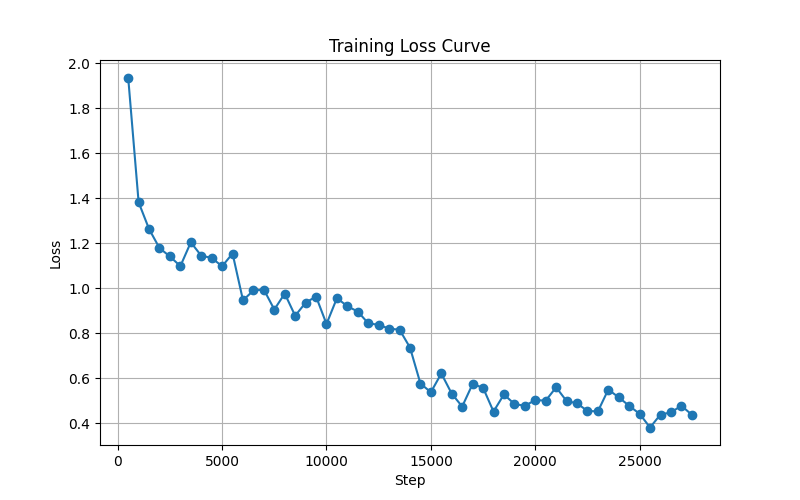
\includegraphics[width=0.7\linewidth]{training_loss_curve.png}
    \caption{Learning curve of the training loss for the span selection (extractive QA) model.}
    \label{fig:training_loss_curve}
\end{figure}


\section{Report - Q4: Pre-trained vs Not Pre-trained (2\%)}
\begin{itemize}
    \item Train a transformer-based model (you can choose either paragraph selection or span selection) from scratch (i.e. without pretrained weights).
    \item Describe
          \begin{itemize}
              \item The configuration of the model and how do you train this model (e.g., hyper-parameters).
              \item The performance of this model v.s. BERT.
          \end{itemize}
    \item Hint
          \begin{itemize}
              \item You can use the same training code, just skip the part where you load the pretrained weights.
              \item The model size configuration for BERT might be too large for this problem, if you find it hard to train a model of the same size, try to reduce model size (e.g. num\_layers, hidden\_dim, num\_heads).
          \end{itemize}
\end{itemize}

\begin{itemize}
    \item Optimizer: AdamW
    \item Learning rate: $5 \times 10^{-4}$
    \item Batch size: 2 (gradient accumulation = 2)
    \item Epochs: 1 (more epochs required due to lack of pretraining)
    \item \textbf{Performance comparison.}
    
    On the validation set, the pretrained \texttt{bert-base-chinese} model reached an accuracy of \textbf{0.9541}, while the scratch-trained model only achieved \textbf{0.5344}. This large gap demonstrates the importance of large-scale language pretraining. The pretrained model benefits from rich linguistic knowledge, enabling it to quickly adapt to the downstream task, whereas the scratch model struggles to learn both the language representation and the task simultaneously from limited data.
\end{itemize}

\section{Report - Q5: Bonus (2\%)}
\begin{itemize}
    \item Instead of the paragraph selection + span selection pipeline approach, train an end-to-end transformer-based model and describe
          Your model.
    \item The performance of your model.
    \item The loss function you used.
    \item The optimization algorithm (e.g. Adam), learning rate and batch size.
    \item Hint: Try models that can handle long input (e.g., models that have a larger context windows).
\end{itemize}

Instead of using the traditional two-step pipeline of paragraph selection followed by span selection, one can consider training an end-to-end transformer-based model that directly predicts the answer span from the entire context. This approach has the advantage of simplifying the architecture and potentially capturing richer interactions between the question and the context.

\subsection{Possible Model}
A suitable model for this task could be a transformer architecture designed to handle long sequences, such as:
\begin{itemize}
    \item Longformer or BigBird for processing longer context windows efficiently.
    \item Pretrained language models like \texttt{hfl/chinese-lert-base} with modifications to extend the maximum input length.
    \item T5 or BART variants that can be fine-tuned in a generative question-answering manner.
\end{itemize}

\subsection{Expected Performance}
The performance of such an end-to-end model is expected to be competitive with the pipeline approach, with potential improvements in cases where paragraph selection errors propagate in the two-step method. Exact Match (EM) and F1 score would be the primary evaluation metrics, similar to standard extractive QA benchmarks like SQuAD.

\subsection{Loss Function}
The standard loss function is the sum of two cross-entropy losses:
\begin{itemize}
    \item Start position loss: cross-entropy between predicted and true start token indices.
    \item End position loss: cross-entropy between predicted and true end token indices.
\end{itemize}
The total loss is typically the average of these two components.

\subsection{Optimization}
The model can be trained using AdamW optimizer with a learning rate of $2\times 10^{-5}$ to $5\times 10^{-5}$, depending on the dataset size. A small batch size (e.g., 1--8 per GPU) is often used for large models due to memory constraints. Gradient accumulation can be applied to simulate larger batch sizes if necessary.

\subsection{Notes on Implementation}
\begin{itemize}
    \item Handling very long contexts may require segmenting the input and using attention mechanisms optimized for long sequences.
    \item End-to-end training simplifies the inference pipeline but may require more GPU memory compared to a pipeline approach.
    \item Techniques like mixed precision training (FP16) and gradient checkpointing can be employed to manage memory usage.
\end{itemize}


% \citep{rajpurkar2018know}

% \section*{Team contributions (Required for multi-person team)}
% Provide a brief summary of what each team member did for the project (about 1 or 2 sentences per person).

% \bibliographystyle{unsrt}
% \bibliography{references}

% \appendix

% \section{Appendix (optional)}
% If you wish, you can include an appendix, which should be part of the main PDF, and does not count towards the 6-8 page limit.
% Appendices can be useful to supply extra details, examples, figures, results, visualizations, etc., that you couldn't fit into the main paper. However, your grader \textit{does not} have to read your appendix, and you should assume that you will be graded based on the content of the main part of your paper only.

\end{document}
